\documentclass[12pt]{beamer}
\usepackage[utf8]{inputenc}
\usetheme{default}
\usepackage{pgf,pgfarrows,pgfnodes}
\usepackage{graphicx}
\usepackage{algorithmicx} 
\usepackage{color}
\usepackage{lipsum}  
\usepackage{xcolor}
\usepackage{hyperref}
\usepackage{ragged2e}
\usepackage{tikz}
\usepackage{multirow}
\usepackage{tabularx}
\usepackage{array}
\usepackage{mathptmx}       % selects Times Roman as basic font
\usepackage{helvet}         % selects Helvetica as sans-serif font
\usepackage{courier}        % selects Courier as typewriter font
\usepackage{type1cm}        % activate if the above 3 fonts are
\usepackage{textpos} 
\usepackage{pgf,pgfarrows,pgfnodes}
\usepackage{graphicx}
\usepackage{color}
\usepackage{natbib}
\setbeamersize{text margin left=10pt,text margin right=10pt}
\definecolor{idrbt_dark_blue}{HTML}{3333b3}
\definecolor{idrbt_blue}{HTML}{00AEEF} 
\definecolor{adroit_black}{HTML}{222222}
\let\oldcite=\cite                                                              
\renewcommand{\cite}[1]{\textcolor[rgb]{0,.7,0}{\oldcite{#1}}}
\setbeamercolor{item}{fg=idrbt_blue}
\setbeamertemplate{section in toc}
{\leavevmode\leftskip=2ex%
	\llap{%
		\usebeamerfont*{section number projected}%
		\usebeamercolor{section number projected}%
		\begin{pgfpicture}{-1ex}{0ex}{1ex}{2ex}
			\color{idrbt_blue}
			%      \color{red}
			\pgfpathcircle{\pgfpoint{0pt}{.75ex}}{1.7ex}
			\pgfusepath{fill}
			\pgftext[base]{\color{fg}\inserttocsectionnumber}
		\end{pgfpicture}\kern1.25ex%
	}%
	\inserttocsection\par}
\date{}
\title{\textcolor{idrbt_blue}{\rule{112mm}{1.25mm}} \textbf{Lecture-1: Introduction to \LaTeX{}}
	 \textcolor{idrbt_blue}{\rule{112mm}{1.25mm}}}
\author{\textcolor{red}{\texttt{\textbf{Manu.V.T.}\\ 
			{\scriptsize Senior Research Fellow\\ Center for Cyber Security\\IDRBT}}} }%\newline {\scriptsize Research Fellow} }
%%%%%%%%%%%%%%%%%%%%%%%%%%%%%%%%%%%%%%%%%%%%%%%%%%%%%%%%%%%%%%
\makeatletter
\long\def\beamer@section[#1]#2{%
	\beamer@savemode%
	\mode<all>%
	\ifbeamer@inlecture
	\refstepcounter{section}%
	\beamer@ifempty{#2}%
	{\long\def\secname{#1}\long\def\lastsection{#1}}%
	{\global\advance\beamer@tocsectionnumber by 1\relax%
		\long\def\secname{#2}%
		\long\def\lastsection{#1}%
		\addtocontents{toc}{\protect\beamer@sectionintoc{\the\c@section}{#2\hfill\the\c@page}{\the\c@page}{\the\c@part}%
			{\the\beamer@tocsectionnumber}}}%
	{\let\\=\relax\xdef\sectionlink{{Navigation\the\c@page}{\noexpand\secname}}}%
	\beamer@tempcount=\c@page\advance\beamer@tempcount by -1%
	\beamer@ifempty{#1}{}{%
		\addtocontents{nav}{\protect\headcommand{\protect\sectionentry{\the\c@section}{#1}{\the\c@page}{\secname}{\the\c@part}}}%
		\addtocontents{nav}{\protect\headcommand{\protect\beamer@sectionpages{\the\beamer@sectionstartpage}{\the\beamer@tempcount}}}%
		\addtocontents{nav}{\protect\headcommand{\protect\beamer@subsectionpages{\the\beamer@subsectionstartpage}{\the\beamer@tempcount}}}%
	}%
	\beamer@sectionstartpage=\c@page%
	\beamer@subsectionstartpage=\c@page%
	\def\insertsection{\expandafter\hyperlink\sectionlink}%
	\def\insertsubsection{}%
	\def\insertsubsubsection{}%
	\def\insertsectionhead{\hyperlink{Navigation\the\c@page}{#1}}%
	\def\insertsubsectionhead{}%
	\def\insertsubsubsectionhead{}%
	\def\lastsubsection{}%
	\Hy@writebookmark{\the\c@section}{\secname}{Outline\the\c@part.\the\c@section}{2}{toc}%
	\hyper@anchorstart{Outline\the\c@part.\the\c@section}\hyper@anchorend%
	\beamer@ifempty{#2}{\beamer@atbeginsections}{\beamer@atbeginsection}%
	\fi%
	\beamer@resumemode}%

\def\beamer@subsection[#1]#2{%
	\beamer@savemode%
	\mode<all>%
	\ifbeamer@inlecture%
	\refstepcounter{subsection}%
	\beamer@ifempty{#2}{\long\def\subsecname{#1}\long\def\lastsubsection{#1}}
	{%
		\long\def\subsecname{#2}%
		\long\def\lastsubsection{#1}%
		\addtocontents{toc}{\protect\beamer@subsectionintoc{\the\c@section}{\the\c@subsection}{#2\hfill\the\c@page}{\the\c@page}{\the\c@part}{\the\beamer@tocsectionnumber}}%
	}%
	\beamer@tempcount=\c@page\advance\beamer@tempcount by -1%
	\addtocontents{nav}{%
		\protect\headcommand{\protect\beamer@subsectionentry{\the\c@part}{\the\c@section}{\the\c@subsection}{\the\c@page}{\lastsubsection}}%
		\protect\headcommand{\protect\beamer@subsectionpages{\the\beamer@subsectionstartpage}{\the\beamer@tempcount}}%
	}%
	\beamer@subsectionstartpage=\c@page%
	\edef\subsectionlink{{Navigation\the\c@page}{\noexpand\subsecname}}%
	\def\insertsubsection{\expandafter\hyperlink\subsectionlink}%
	\def\insertsubsubsection{}%
	\def\insertsubsectionhead{\hyperlink{Navigation\the\c@page}{#1}}%
	\def\insertsubsubsectionhead{}%
	\Hy@writebookmark{\the\c@subsection}{#2}{Outline\the\c@part.\the\c@section.\the\c@subsection.\the\c@page}{3}{toc}%
	\hyper@anchorstart{Outline\the\c@part.\the\c@section.\the\c@subsection.\the\c@page}\hyper@anchorend%
	\beamer@ifempty{#2}{\beamer@atbeginsubsections}{\beamer@atbeginsubsection}%
	\fi%
	\beamer@resumemode}

\makeatother
%%%%%%%%%%%%%%%%%%%%%%%%%%%%%%%%%%%%%%%%%%%%%%%%%%%%%%%%%%%%%%
\beamertemplatenavigationsymbolsempty

\addtobeamertemplate{navigation symbols}{}{%
	\usebeamerfont{footline}%
	\usebeamercolor[fg]{footline}%
	\hspace{1em}%
	\insertframenumber/\inserttotalframenumber
}
%%%%%%%%%%%%%%%%%%%%%%%%%%%%%%%%%%%%%%%%%%%%%%%%%%%%%%%%%%%%%%
\begin{document}
	%%%%%%%%%%%%%%%%%%%%%%%%%%%%%%%%%%%%%%%%%%%%%%%%%%%%%%%%%%%%%%%%%%%%%%%%%%%%%%%%%%%%%%%%%%%%%%%%%%%%%%%%%%%%%%%%%%%%%%%%%%%%%
	\begin{frame}
	\titlepage
	


\begin{center}
			\begin{tabular}{l>{\centering}p{6.25cm}<{\centering}l}
			\multirow{1}{*}{
\includegraphics[scale=0.15]{./IDRBT_lowres.png}}
			&
         
			&
			\multirow{1}{*}{
\includegraphics[scale=0.25]{./uoh.png}}
		\end{tabular}
\end{center}

\smallskip
	\renewcommand*{\arraystretch}{1.05}



\end{frame}
%%%%%%%%%%%%%%%%%%%%%%%%%%%%%%%%%%%%%%%%%%%%%%%%%%%%%%%%%%%%%%%%%%%%%%%%%%%%%%%%%%%%%%%%%%%%%%%%%%%%%%%%%%%%%%%%%%%%%%%%%%%%%

\begin{frame}
\frametitle{Outline}
\tableofcontents %[hideallsubsections]
\end{frame}
%%%%%%%%%%%%%%%%%%%%%%%%%%%%%%%%%%%%%%%%%%%%%%%%%%%%%%%%%%%%%%%%%%%%%%%%%%%%%%%%%%%%%%%%%%%%%%%%%%%%%%%%%%%%%%%%%%%%%%%%%%%%%

%%%%%%%%%%%%%%%%%%%%%%%%%%%%%%%%%%%%%%%%%%%%%%%%%%%%%%%%%%%%%%%%%%%%%%%%%%%%%%%%%%%%%%%%%%%%%%%%%%%%%%%%%%%%%%%%%%%%%%%%%%%%%
\begin{frame}
\section{ What is \TeX?}
\frametitle{ What is \TeX?}
\begin{itemize}\justifying
	\item A low-level markup and programming language created by \textbf{Donald Knuth} to
	typeset documents attractively and consistently.
	\item Programming language- 
	\begin{itemize}\justifying
		\item Supports the if-else construct: you can make calculations with it (that
		are performed while compiling the document), etc.
		\item Find it very hard to do
		anything else but typesetting with it.
	\end{itemize}
\item Very gradual learning curve, requiring
a significant investment of time to build custom macros for text formatting.
\end{itemize}
\end{frame}
%%%%%%%%%%%%%%%%%%%%%%%%%%%%%%%%%%%%%%%%%%%%%%%%%%%%%%%%%%%%%%%%%%%%%%%%%%%%%%%%%%%%%%%%%%%%%%%%%%%%%%%%%%%%%%%%%%%%%%%%%%%%%
%%%%%%%%%%%%%%%%%%%%%%%%%%%%%%%%%%%%%%%%%%%%%%%%%%%%%%%%%%%%%%%%%%%%%%%%%%%%%%%%%%%%%%%%%%%%%%%%%%%%%%%%%%%%%%%%%%%%%%%%%%%%%
\begin{frame}
\section{ What is \LaTeX?}
\frametitle{ What is \LaTeX?}
\begin{itemize}\justifying
	\item Pre-built macros are time saving, and automate certain repetitive tasks and
	help reduce user introduced errors; however, this convenience comes at the cost of complete
	design flexibility. 
	\item One of the most popular macro packages is called \LaTeX	
\end{itemize}
\end{frame}
%%%%%%%%%%%%%%%%%%%%%%%%%%%%%%%%%%%%%%%%%%%%%%%%%%%%%%%%%%%%%%%%%%%%%%%%%%%%%%%%%%%%%%%%%%%%%%%%%%%%%%%%%%%%%%%%%%%%%%%%%%%%%
 \begin{frame}
 \frametitle{Why \LaTeX \hspace{1pt} Over Word Processors?}
\begin{itemize}\justifying
	\item Manual formatting of a document,
	as usually required in many word processors, can be automated in \LaTeX. 
	\item Possibility of doing any mistake in numbering and referring items (sections,
	tables, figures or equations), in choosing size and type of fonts for different sections
	and subsections, or in preparing bibliographic references, can be avoided. 
	\item Has the provision for automatically generating various lists of contents, index,
	and glossary. 
\end{itemize}
\end{frame}
%%%%%%%%%%%%%%%%%%%%%%%%%%%%%%%%%%%%%%%%%%%%%%%%%%%%%%%%%%%%%%%%%%%%%%%%%%%%%%%%%%%%%%%%%%%%%%%%%%%%%%%%%%%%%%%%%%%%%%%%%%%%%
\begin{frame}
\section{ Basic Installation \& Initial Configuration}
\frametitle{ Basic Installation \& Initial Configuration}	
\begin{itemize}\justifying
	\item GNU$\backslash$Linux $\rightarrow$ TeXLive (basic system) \& texlive-extra (additional features, fonts, etc)
	\item Windows $\rightarrow$ MiKTeX
\end{itemize}
Preferred IDEs
\begin{itemize}
	\item TeXstudio : Both on Windows and GNU $\backslash$ Linux
	\item Gummi, Kile : GNU $\backslash$ Linux
\end{itemize}
If comfortable with command prompt/ shell 
\begin{itemize}
	\item Vim, Geany : GNU $\backslash$ Linux
	\item Notepad++ : Windows
\end{itemize}
\end{frame}

\begin{frame}			
\section{ Basics of \LaTeX	}	
\frametitle{ Basics of \LaTeX	}	
\begin{center}
	
\includegraphics[width=0.7\linewidth]{lion}
\end{center}

\end{frame}
%%%%%%%%%%%%%%%%%%%%%%%%%%%%%%%%%%%%%%%%%%%%%%%%%%%%%%%%%%%%%%%%%%%%%%%%%%%%%%%%%%%%%%%%%%%%%%%%%%%%%%%%%%%%%%%%%%%%%%%%%%%%%
\begin{frame}			
\frametitle{How to Prepare a \LaTeX \hspace{1pt} Input File?}
\begin{center}
		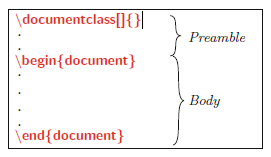
\includegraphics[scale=0.5]{first_file}
\end{center}
\end{frame}
%%%%%%%%%%%%%%%%%%%%%%%%%%%%%%%%%%%%%%%%%%%%%%%%%%%%%%%%%%%%%%%%%%%%%%%%%%%%%%%%%%%%%%%%%%%%%%%%%%%%%%%%%%%%%%%%%%%%%%%%%%%%%
%%%%%%%%%%%%%%%%%%%%%%%%%%%%%%%%%%%%%%%%%%%%%%%%%%%%%%%%%%%%%%%%%%%%%%%%%%%%%%%%%%%%%%%%%%%%%%%%%%%%%%%%%%%%%%%%%%%%%%%%%%%%%
\begin{frame}		
\section{ How to Compile a \LaTeX Input File?}	
\frametitle{ How to Compile a \LaTeX Input File?}
\begin{itemize}\justifying
	\item .tex file 
	\item pdflatex creates a PDF, .aux, .log
\end{itemize}
\end{frame}
%%%%%%%%%%%%%%%%%%%%%%%%%%%%%%%%%%%%%%%%%%%%%%%%%%%%%%%%%%%%%%%%%%%%%%%%%%%%%%%%%%%%%%%%%%%%%%%%%%%%%%%%%%%%%%%%%%%%%%%%%%%%%
\begin{frame}
\frametitle{\LaTeX Syntax}
\begin{itemize}
	\item commands : usually starts with a $\backslash$
	\item environment
	\item packages
\end{itemize}
\end{frame}
%%%%%%%%%%%%%%%%%%%%%%%%%%%%%%%%%%%%%%%%%%%%%%%%%%%%%%%%%%%%%%%%%%%%%%%%%%%%%%%%%%%%%%%%%%%%%%%%%%%%%%%%%%%%%%%%%%%%%%%%%%%%%
\begin{frame}\frametitle{Special Characters}
\begin{center}
	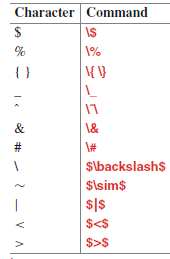
\includegraphics[scale=0.5]{special_Characters}
\end{center}

\end{frame}
%%%%%%%%%%%%%%%%%%%%%%%%%%%%%%%%%%%%%%%%%%%%%%%%%%%%%%%%%%%%%%%%%%%%%%%%%%%%%%%%%%%%%%%%%%%%%%%%%%%%%%%%%%%%%%%%%%%%%%%%%%%%%
\begin{frame}[fragile]			
\section{ Creating First Document}	
\frametitle{ Creating First Document}			
\begin{verbatim}
\documentclass[]{article}
\begin{document} 
Hello World! 
\end{document}
\end{verbatim}
\end{frame}
%%%%%%%%%%%%%%%%%%%%%%%%%%%%%%%%%%%%%%%%%%%%%%%%%%%%%%%%%%%%%%%%%%%%%%%%%%%%%%%%%%%%%%%%%%%%%%%%%%%%%%%%%%%%%%%%%%%%%%%%%%%%%
\begin{frame}[fragile]			
\frametitle{ Fonts Selection}			
\begin{itemize}\justifying
	\item Text-Mode Fonts
	\begin{itemize}
		\item The default font type of a \LaTeX{} document is medium series serif family in upright
		shape and 10 pt size. 
		\item The sizes of fonts in different parts of a document, say in headings and in paragraphs, are calculated proportionately.
		\item The default font setting can be altered globally through various options
		to the 
		\begin{verbatim}
		\documentclass[ ]{ }
		\end{verbatim} command, e.g.,
		\begin{verbatim}
		 \documentclass[12pt]{article}
		\end{verbatim} for producing
		an article in 12 pt fonts.
	\end{itemize}
	\item \LaTeX{} Menu in the IDE
\end{itemize}
\end{frame}
%%%%%%%%%%%%%%%%%%%%%%%%%%%%%%%%%%%%%%%%%%%%%%%%%%%%%%%%%%%%%%%%%%%%%%%%%%%%%%%%%%%%%%%%%%%%%%%%%%%%%%%%%%%%%%%%%%%%%%%%%%%%%

%%%%%%%%%%%%%%%%%%%%%%%%%%%%%%%%%%%%%%%%%%%%%%%%%%%%%%%%%%%%%%%%%%%%%%%%%%%%%%%%%%%%%%%%%%%%%%%%%%%%%%%%%%%%%%%%%%%%%%%%%%%%%
\begin{frame}[fragile]			
\section{ Sectional Units}	
\frametitle{ Sectional Units}			
\begin{itemize}\justifying
	\item Various sectional units, like chapters and sections, are generated using 
	\begin{verbatim}
	\chapter{ }, \section{ }, \subsection{ }, 
	\subsubsection{ }, \paragraph{ } &
	\subparagraph{ } 
	\end{verbatim}
	\item

		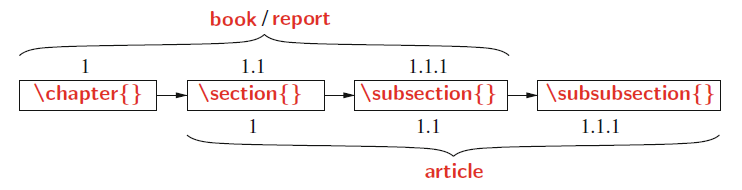
\includegraphics[scale=0.45]{Sectioning}

	
\end{itemize}
\end{frame}
%%%%%%%%%%%%%%%%%%%%%%%%%%%%%%%%%%%%%%%%%%%%%%%%%%%%%%%%%%%%%%%%%%%%%%%%%%%%%%%%%%%%%%%%%%%%%%%%%%%%%%%%%%%%%%%%%%%%%%%%%%%%%
\begin{frame}[fragile]			
\section{Labeling and Referring Example}	
\frametitle{Labeling and Referring Example}			
\begin{verbatim}
\section{About Me}\label{sec:cg}
\end{verbatim}
Hi today is our introduction class on \LaTeX.
I am Manu VT and I work with Prof.Mehtre.
Before joining for PhD, I was teaching in NIT Calicut for sometime.
\begin{verbatim}
\subsection{Trivia}\label{sec:sb}
\end{verbatim}
I am from Kerala. People say it is ''God's Own Country'', but only a few know that it is the tag line of The Kerala Tourism Project. 
\begin{verbatim}
\section{More About Me}\label{sec:ex}
\end{verbatim}
My name and PhD thesis advisor's names are mentioned in Section.\verb|\ref{sec:cg}|.
Information about my native place is given in  \verb|\ref{sec:sb}|.
\end{frame}
%%%%%%%%%%%%%%%%%%%%%%%%%%%%%%%%%%%%%%%%%%%%%%%%%%%%%%%%%%%%%%%%%%%%%%%%%%%%%%%%%%%%%%%%%%%%%%%%%%%%%%%%%%%%%%%%%%%%%%%%%%%%%
\begin{frame}\frametitle{\LaTeX{} Output}	
\begin{flushleft}
	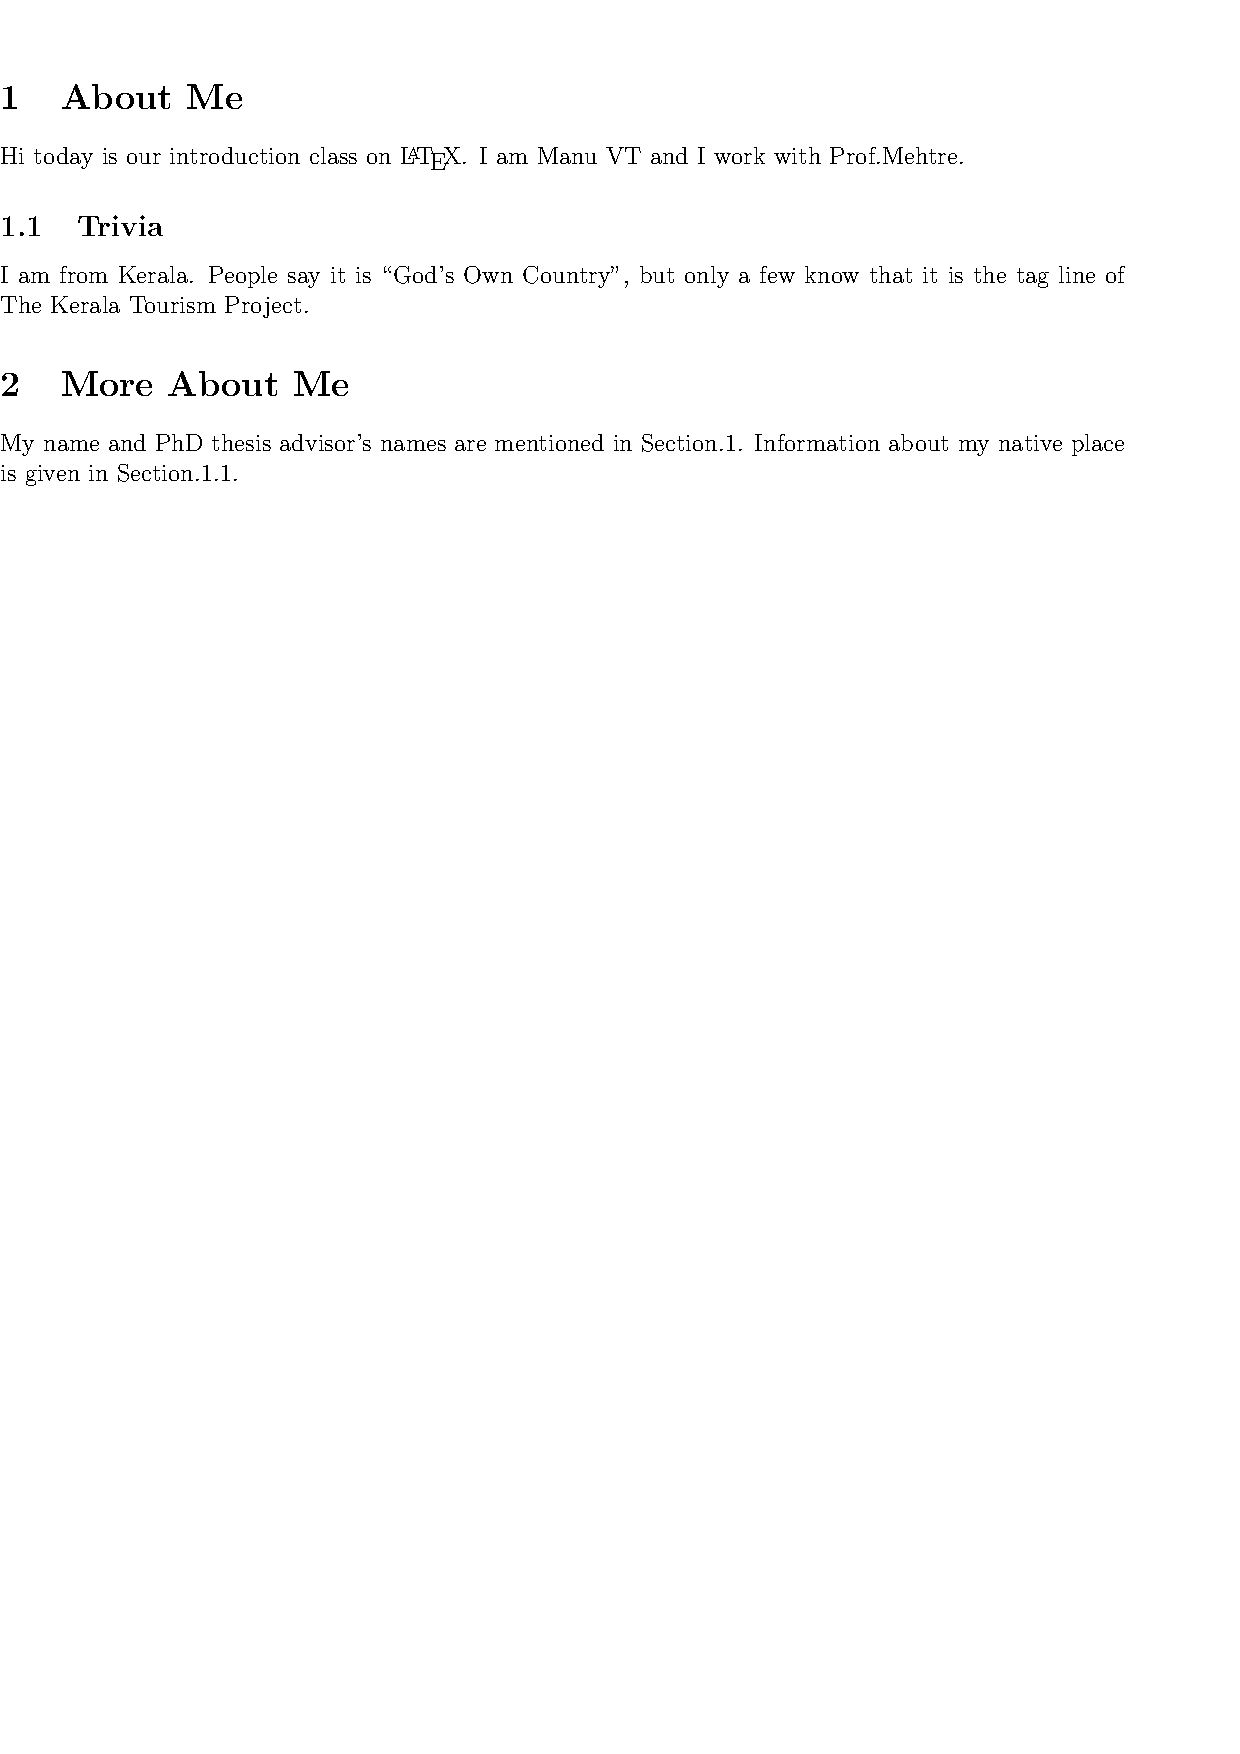
\includegraphics[scale=0.6]{example}
\end{flushleft}
\end{frame}
%%%%%%%%%%%%%%%%%%%%%%%%%%%%%%%%%%%%%%%%%%%%%%%%%%%%%%%%%%%%%%%%%%%%%%%%%%%%%%%%%%%%%%%%%%%%%%%%%%%%%%%%%%%%%%%%%%%%%%%%%%%%%

%%%%%%%%%%%%%%%%%%%%%%%%%%%%%%%%%%%%%%%%%%%%%%%%%%%%%%%%%%%%%%%%%%%%%%%%%%%%%%%%%%%%%%%%%%%%%%%%%%%%%%%%%%%%%%%%%%%%%%%%%%%%%
\begin{frame}[fragile]
\frametitle{ Customizing Page Layouts (Contd...)}
\begin{verbatim}
\topmargin -0.5in
\headheight 0in
\headsep 0in
\textheight 12in
\textwidth 6.5in
\oddsidemargin 0in
\evensidemargin 0in
\pagenumbering{gobble}
\end{verbatim}
\end{frame}
%%%%%%%%%%%%%%%%%%%%%%%%%%%%%%%%%%%%%%%%%%%%%%%%%%%%%%%%%%%%%%%%%%%%%%%%%%%%%%%%%%%%%%%%%%%%%%%%%%%%%%%%%%%%%%%%%%%%%%%%%%%%%
\begin{frame}[fragile]			
\frametitle{ Texts Alignment}
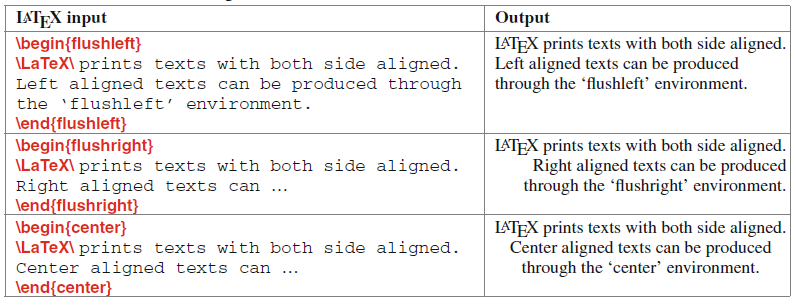
\includegraphics[width=1\linewidth]{TextAlignment}
\end{frame}
%%%%%%%%%%%%%%%%%%%%%%%%%%%%%%%%%%%%%%%%%%%%%%%%%%%%%%%%%%%%%%%%%%%%%%%%%%%%%%%%%%%%%%%%%%%%%%%%%%%%%%%%%%%%%%%%%%%%%%%%%%%%%
\begin{frame}[fragile]			
\frametitle{ Listing Texts}
\begin{itemize}
	\item  itemize
		\begin{verbatim} 
		\begin{itemize}
		\item Raghu
		\item Sridevi
		\item Nanatlam
		\end{itemize}
		\end{verbatim}
	\item  enumerate
		\begin{verbatim}
			\begin{enumerate}
			\item Raghu
			\item Sridevi
			\end{enumerate}
		\end{verbatim}
	\item  description		
		\begin{verbatim}
		\begin{description}
				\item[Raghu] He is a research fellow
			\item[Nanatlam] He is liked to be called NDP
		\end{description}
		\end{verbatim} 
\end{itemize}
\end{frame}

\begin{frame}
\frametitle{ Listing Texts}

		\begin{itemize}
	\item Raghu
	\item Sridevi
	\item Nanatlam
\end{itemize}

			\begin{enumerate}
	\item Raghu
	\item Sridevi
\end{enumerate}

		\begin{description}
	\item[Raghu] He is a research fellow
	\item[Nanatlam] He is liked to be called NDP
\end{description}

\end{frame}
%%%%%%%%%%%%%%%%%%%%%%%%%%%%%%%%%%%%%%%%%%%%%%%%%%%%%%%%%%%%%%%%%%%%%%%%%%%%%%%%%%%%%%%%%%%%%%%%%%%%%%%%%%%%%%%%%%%%%%%%%%%%%
\begin{frame}
 \begin{center}
\begin{block}{}
\hspace*{2in}\textbf{\LARGE \textcolor{idrbt_dark_blue}{T}\pause
			    \textcolor{idrbt_blue}{h}\pause
			    \textcolor{idrbt_dark_blue}{a}\pause
			    \textcolor{idrbt_blue}{n}\pause
			    \textcolor{idrbt_dark_blue}{k}\pause
			    \textcolor{idrbt_dark_blue}{Y}\pause
			    \textcolor{idrbt_blue}{o}\pause
			    \textcolor{idrbt_dark_blue}{u} }
\end{block}\end{center}
\end{frame}
\end{document}
%%%%%%%%%%%%%%%%%%%%%%%%%%%%%%%%%%%%%%%%%%%%%%%%%%%%%%%%%%%%%%%%%%%%%%%%%%%%%%%%%%%%%%%%%%%%%%%%%%%%%%%%%%%%%%%%%%%%%%%%%%%%%